\documentclass[12pt,twoside]{report}

% some definitions for the title page
\newcommand{\reporttitle}{Transfer Learning for Deep Learning Radiotherapy Planning}
\newcommand{\reportauthor}{Anton Zhitomirsky}
\newcommand{\supervisor}{Prof Ben Glocker}
\newcommand{\secondMarker}{Dr Thomas Heinis}
\newcommand{\reporttype}{MEng Individual Project}

% load some definitions and default packages
%%%%%%%%%%%%%%%%%%%%%%%%%%%%%%%%%%%%%%%%%
% University Assignment Title Page 
% LaTeX Template
% Version 1.0 (27/12/12)
%
% This template has been downloaded from:
% http://www.LaTeXTemplates.com
%
% Original author:
% WikiBooks (http://en.wikibooks.org/wiki/LaTeX/Title_Creation)
%
% License:
% CC BY-NC-SA 3.0 (http://creativecommons.org/licenses/by-nc-sa/3.0/)
% 
%
%%%%%%%%%%%%%%%%%%%%%%%%%%%%%%%%%%%%%%%%%
%----------------------------------------------------------------------------------------
%	PACKAGES AND OTHER DOCUMENT CONFIGURATIONS
%----------------------------------------------------------------------------------------
\usepackage[a4paper,hmargin=2.0cm,vmargin=1.0cm,includeheadfoot]{geometry}
\usepackage{textpos}

\usepackage[square,numbers]{natbib} % for bibliography
\usepackage[nottoc]{tocbibind} % Includes "References" in the table of contents
\bibliographystyle{unsrtnat}

\usepackage{tabularx,longtable,multirow,subfigure,caption}%hangcaption
\usepackage{fancyhdr} % page layout
\usepackage{url} % URLs
\usepackage[english]{babel}
\usepackage{amsmath}
\usepackage{graphicx}
\usepackage{scalerel}
\usepackage{dsfont}
\usepackage{epstopdf} % automatically replace .eps with .pdf in graphics
\usepackage{backref} % needed for citations
\usepackage{array}
\usepackage{latexsym}

\usepackage[pdftex,pagebackref,hypertexnames=false,colorlinks]{hyperref} % provide links in pdf
\usepackage{booktabs}
\usepackage{wrapfig}
\usepackage{caption}  % Required for \captionof
\usepackage{float} % for H option in figures
\usepackage{amssymb}
\usepackage{amsmath}
\usepackage{csquotes}
% \usepackage{subcaption} % causes a compilation error after changing back to natbib referencing... 

\hypersetup{pdftitle={},
  pdfsubject={}, 
  pdfauthor={},
  pdfkeywords={}, 
  pdfstartview=FitH,
  pdfpagemode={UseOutlines},% None, FullScreen, UseOutlines
  bookmarksnumbered=true, bookmarksopen=true, colorlinks,
    citecolor=black,%
    filecolor=black,%
    linkcolor=black,%
    urlcolor=black}

\usepackage[all]{hypcap}

%%%%%%%%%%%%%%%%%%%%%%%%%%%%%%%%%%%%%%%%%%%%%%%%%%%%%%%%%%%%%%%%%%%%%%%%%%%%%%%%
% LISTINGS ammendments
%%%%%%%%%%%%%%%%%%%%%%%%%%%%%%%%%%%%%%%%%%%%%%%%%%%%%%%%%%%%%%%%%%%%%%%%%%%%%%%%
\usepackage{listings}

\lstset
{ %Formatting for code in appendix
    language=Matlab,
    basicstyle=\footnotesize,
    % numbers=left,
    stepnumber=1,
    showstringspaces=false,
    tabsize=1,
    breaklines=true,
    breakatwhitespace=false,
    frame=single,
    columns=fullflexible,
    postbreak=\mbox{\textcolor{red}{$\hookrightarrow$}\space},
}

%\usepackage{color}
%\usepackage[tight,ugly]{units}
%\usepackage{float}
%\usepackage{tcolorbox}
%\usepackage[colorinlistoftodos]{todonotes}
% \usepackage{ntheorem}
% \theoremstyle{break}
% \newtheorem{lemma}{Lemma}
% \newtheorem{theorem}{Theorem}
% \newtheorem{remark}{Remark}
% \newtheorem{definition}{Definition}
% \newtheorem{proof}{Proof}


%%% Default fonts
\renewcommand*{\rmdefault}{bch}
\renewcommand*{\ttdefault}{cmtt}


%%% Default settings (page layout)
\setlength{\parindent}{0em}  % indentation of paragraph
\setlength{\parskip}{.3em}

% \setlength{\parindent}{0em}  % indentation of paragraph

\setlength{\headheight}{14.5pt}
\pagestyle{fancy}
\renewcommand{\chaptermark}[1]{\markboth{\chaptername\ \thechapter.\ #1}{}}
%\fancyhead[RO]{\sffamily \textbf{\thepage}} %Page no.in the right on even pages
%\fancyhead[LE]{\sffamily \textbf{\thepage}} %Page no. in the left on odd pages

\fancyfoot[ER,OL]{\thepage}%Page no. in the left on
%odd pages and on right on even pages
\fancyfoot[OC,EC]{\sffamily }
\renewcommand{\headrulewidth}{0.1pt}
\renewcommand{\footrulewidth}{0.1pt}
\captionsetup{margin=10pt,font=small,labelfont=bf}


%--- chapter heading

\def\@makechapterhead#1{%
  \vspace*{10\p@}%
  {\parindent \z@ \raggedright \sffamily
    \interlinepenalty\@M
    \Huge\bfseries \thechapter \space\space #1\par\nobreak
    \vskip 30\p@
  }}

%--- chapter heading

\def\@makechapterhead#1{%
  \vspace*{10\p@}%
  {\parindent \z@ \raggedright \sffamily
    %{\Large \MakeUppercase{\@chapapp} \space \thechapter}
    %\\
    %\hrulefill
    %\par\nobreak
    %\vskip 10\p@
    \interlinepenalty\@M
    \Huge\bfseries \thechapter \space\space #1\par\nobreak
    \vskip 30\p@
  }}

%---chapter heading for \chapter*  
\def\@makeschapterhead#1{%
  \vspace*{10\p@}%
  {\parindent \z@ \raggedright
    \sffamily
    \interlinepenalty\@M
    \Huge \bfseries  #1\par\nobreak
    \vskip 30\p@
  }}
\allowdisplaybreaks

% load some macros
% Here, you can define your own macros. Some examples are given below.

\newcommand{\R}[0]{\mathds{R}} % real numbers
\newcommand{\Z}[0]{\mathds{Z}} % integers
\newcommand{\N}[0]{\mathds{N}} % natural numbers
\newcommand{\C}[0]{\mathds{C}} % complex numbers
% \renewcommand{\vec}[1]{{\boldsymbol{{#1}}}} % vector
\newcommand{\mat}[1]{{\boldsymbol{{#1}}}} % matrix

\usepackage{pifont,mdframed}
\newenvironment{warning}
  {\par\begin{mdframed}[linewidth=1pt,linecolor=black]%
    \begin{list}{}{\leftmargin=1cm
                  \labelwidth=\leftmargin}\item[\Large\ding{43}]}
  {\end{list}\end{mdframed}\par}

\definecolor{lightgray}{gray}{0.9}

% load title page
\begin{document}
% Last modification: 2015-08-17 (Marc Deisenroth)
\begin{titlepage}

    \newcommand{\HRule}{\rule{\linewidth}{0.5mm}} % Defines a new command for the horizontal lines, change thickness here
    
    %----------------------------------------------------------------------------------------
    %	LOGO SECTION
    %----------------------------------------------------------------------------------------
    
    
\includegraphics[width = 4cm]{../figures/imperial.pdf}\\[0.5cm] 
    
    \center % Center everything on the page
     
    %----------------------------------------------------------------------------------------
    %	HEADING SECTIONS
    %----------------------------------------------------------------------------------------
    
    \textsc{\LARGE \reporttype}\\[1.5cm] 
    \textsc{\Large Department of Computing}\\[0.5cm] 
    \textsc{\large Imperial College of Science, Technology and Medicine}\\[0.5cm] 
    
    %----------------------------------------------------------------------------------------
    %	TITLE SECTION
    %----------------------------------------------------------------------------------------
    
    \HRule \\[0.4cm]
    { \huge \bfseries \reporttitle}\\ % Title of your document
    \HRule \\[1.5cm]
     
    %----------------------------------------------------------------------------------------
    %	AUTHOR SECTION
    %----------------------------------------------------------------------------------------
    
    \begin{minipage}{0.4\textwidth}
    \begin{flushleft} \large
    \emph{Author:}\\
    \reportauthor % Your name
    \end{flushleft}
    \end{minipage}
    ~
    \begin{minipage}{0.4\textwidth}
    \begin{flushright} \large
    \emph{Supervisor:} \\
    \supervisor % Supervisor's Name
    \end{flushright}
    \end{minipage}\\[4cm]
    
    
    
    
    %----------------------------------------------------------------------------------------
    
    
    %----------------------------------------------------------------------------------------
    %	DATE SECTION
    %----------------------------------------------------------------------------------------
    
    {\large \today} % Date, change the \today to a set date if you want to be precise
    
    
    \vfill % Fill the rest of the page with whitespace
    Submitted in partial fulfillment of the requirements for the \degreetype~of Imperial College London
    
    \end{titlepage}
    

% page numbering etc.
\pagenumbering{roman}
\clearpage{\pagestyle{empty}\cleardoublepage}
\setcounter{page}{1}
\pagestyle{fancy}

% \cleardoublepage
%%%%%%%%%%%%%%%%%%%%%%%%%%%%%%%%%%%%
% \section*{Acknowledgments}
% Comment this out if not needed.

% \clearpage{\pagestyle{empty}\cleardoublepage}

%%%%%%%%%%%%%%%%%%%%%%%%%%%%%%%%%%%%

% \begin{abstract}\label{sect:abstract}
   
% \end{abstract}
  
%%%%%%%%%%%%%%%%%%%%%%%%%%%%%%%%%%%%
%--- table of contents
\fancyhead[RE,LO]{\sffamily {Table of Contents}}
\tableofcontents
  
% \clearpage{\pagestyle{empty}\cleardoublepage}

%%%%%%%%%%%%%%%%%%%%%%%%%%%%%%%%%%%%

\pagenumbering{arabic}
\setcounter{page}{1}
\fancyhead[LE,RO]{\slshape \rightmark}
\fancyhead[LO,RE]{\slshape \leftmark}

%%%%%%%%%%%%%%%%%%%%%%%%%%%%%%%%%%%%
\chapter{Introduction}

\section{Technical Context}
\section{Objectives and Contributions}
\section{Outline of Report}

%%%%%%%%%%%%%%%%%%%%%%%%%%%%%%%%%%%%
\chapter{Background}

\section{Clinical Context}

This project will have its foundation for experimentation in a dataset provided by the Royal Marsden Hospital. We introduce this real-world clinical dataset, which has no exposure in academia and has uncommon and limited segmentation patterns, that will act as the pillar for justifying the success and transferability of ideas explored in this project to other medical domains. This dataset segments key anatomies and tumours which aid in radiotherapy planning for females with cervical cancer.

In this section, we discuss the clinical context behind cervical cancer in the population, the Hospital's pipeline for segmenting patients in preparation for radiotherapy treatment, and the Hospital's motivation for recruiting an AI tool to assist in its treatment pipeline. 

\subsection{Cervical Cancer}\label{sect:cervical-cancer}

Cancer is a burden around the globe that has been a driver for almost one-sixth of the world's mortality in 2022~\cite{Global-cancer-2022}. In females, cervical cancer makes up 25 countries' leading causes of cancer death, following breast cancer in 157 in 2022~\cite{Global-cancer-2022}. Furthermore, the resulting maternal orphans from cancers affecting females experience health and education disadvantages throughout their lives~\cite{Guida2022}. Thankfully, cancer screening services provided by hospitals around Europe have been shown to decrease incidence and mortality rates of cervical cancer in women over the recent years~\cite{Global-cancer-2022}, which inspires further complete clinical understanding of the disease. This motivation and the potential to pair with quality improvements offered by medical imaging models drive this research project to explore transfer knowledge in this field.


% In 2017, Cervical Cancer accumulated 530,000 new cases annually, with 270,000 deaths, making it the fourth most common malignancy diagnosed in women worldwide~\cite{cervical-cancer-epidemic}. A common treatment mechanism involves radiation therapy which targets cancerous cells in a clinically defined target area with beams of high energy (Section~\ref{sect:radiotherapy}). This treatment is tedious, as it is estimated that an oncologist needs 90-120 min to delineate target areas for radiotherapy~\cite{LIU2020184}.

% This time consuming nature of studying each patient makes treating cancers a time consuming endeavour which is particularly threatening when time is not on the patients side. Death from Cervical Cancer involves significant pain and suffering for the patients who cannot receive urgent treatment~\cite{cervical-cancer-epidemic}. This is particularly a problem in mid-low income countries with approximately 85\% of cases of cervical cancer occurring, making them have 18 times the death rates of high-income countries~\cite{cervical-cancer-epidemic}. 

% \subsubsection{Radiotherapy}\label{sect:radiotherapy}

% Radiation therapy is a treatment option for cancer treatment. In 2012, approximately 50\% of all cancer patients received radiation therapy, with an additional 40\% involving curative treatment~\cite{radiotherapy-advances}. 

% Physicians abuse the physical properties of radiation to damage the genetic material of cells and block their ability to cause further damage to a patient~\cite{radiotherapy-advances}. Importantly for our cause, radiation damages intercellular molecules leading to degradation and stopping a cells ability to divide, leading to interphase death. Alternatively, radiation may cause a ``mitotic catastrophe'' causing a cell to die of a proliferative death~\cite{cell-death}. 

% \subsubsection{Contour Planning}\label{sect:contour-planning}

% Radiotherapy has become a great option due to high resolution X-ray or CT scans which produce high contrasting images of the damaged and surrounding soft tissue~\cite{radiotherapy-basic-concepts}. Physicians then use this 3D scan to plan a target volume for the radiation therapy surrounding the tumor in hopes of killing it and not damaging the surrounding tissue.

% \subsubsection{Process}

% This begins with the high contrasting image of the tumour area. In a clinical setting, an Oncologist will use knowledge about the particular cancer to determine target structures, structures we need to protect (organs-at-risk), and areas where each particular cancer is likely to spread to~\cite{AMLART-data}. 

% The first area defined from the scan is the Gross Target Volume (GTV). This macroscopic delineated area is the visible tumour area on the scan and contains a high probability of containing the tumour. Secondly, the Clinical Target Volume (CTV) is derived to account for potential microscopic spread. This will be an area at least as big as the tumor area segmented in the GTV with an optional margin surrounding it containing a 'rind' of non-zero probability of tumour spread. Lastly, the Primary Tumour Volume (PTV) contains residual geometric uncertainties and safety margins surrounding the CTV ensuring the radiotherapy dose is actually delivered to the CTV~\cite{tumor-delineation,defining-target-volumes,Lin2021-oz,personalised-PTV-strategies}. These target volumes also constantly consider critical normal tissue structures which need to be preserved during irradiation. These are referred to as organs-at-risk (ORs). In some specific circumstances, it is necessary to add a margin analogous to the PTV margin around an OR to ensure that the organ cannot receive a higher-than-safe dose; this gives a planning organ at risk volume~\cite{defining-target-volumes}.

% \subsubsection{A tangent on Accuracy}

% The CTV volumes may vary between clinicians as there is no internationally agreed guidelines. As a very time consuming process which high variability it therefore suffers from a lot of inter and intra-observer variability~\cite{Lin2021-oz}. However, the data provided has been standardized as a gold standard, see Section~\ref{sect:data}.

% The PTV volume is an additional step which provides a margin of protection surrounding the CTV. One might think that a CTV step is the final step in clinical trials as it defines the most tight volume surrounding the cancerous site, however, geometric errors are impossible to eliminate. This includes short-term organ movement, voxel size and slice resolution, and possibility of relative movement of structure of reference and the tumour~\cite{VANHERK200452}

\subsection{CT modality}

The CT scan is a popular imaging modality in clinical environments because of its non-invasive ability to provide detailed images of the internal structures of the body. A series of X-ray devices are rotated around a specified body part, and computer-generated cross-sectional images are produced~\cite{file-formats}. Whilst the scanner rotates, the table the patient lies on slowly moves up and down inside the tube to produce different cross-section images. 

\subsubsection{Hounsfield Units}

\begin{figure}[H]
    \centering
    \subfigure[Muscle Window $(35,55)$~\cite{other-HD-units}]{{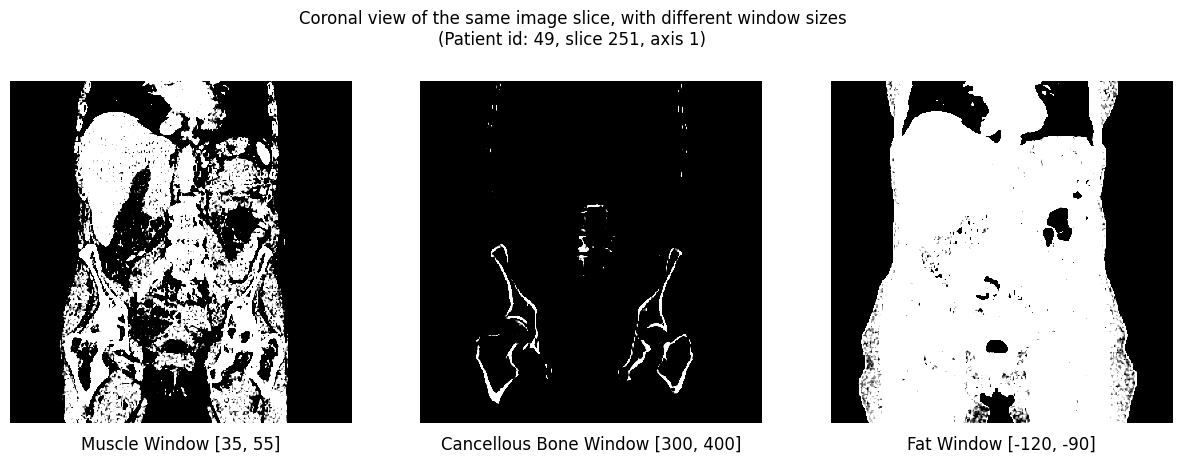
\includegraphics[width=0.3\textwidth, trim=0.2cm 1cm 21cm 2cm, clip]{../figures/HU-window.png}}}
    \subfigure[Cancellous Bone Window  $(300,400)$~\cite{cancellous-bone}]{{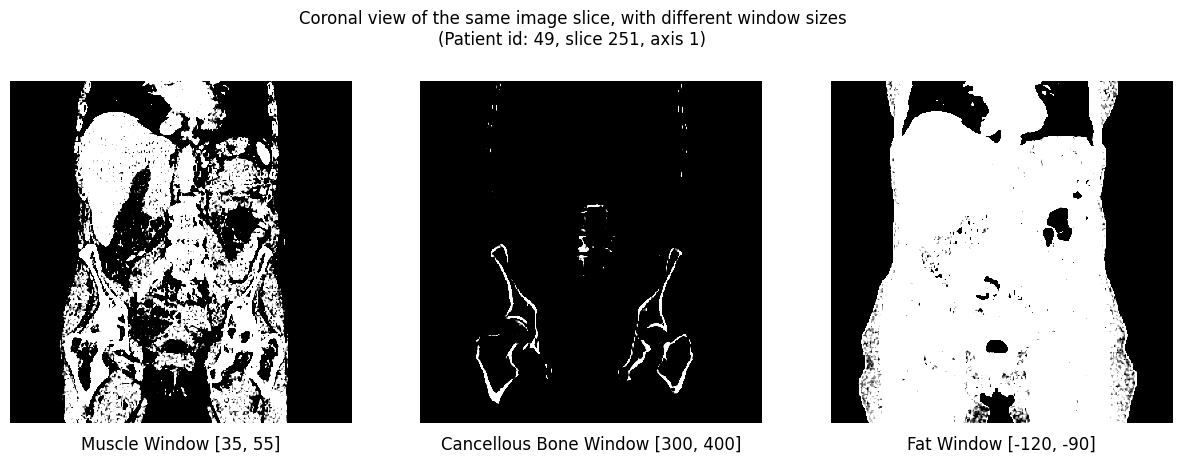
\includegraphics[width=0.3\textwidth, trim=10.6cm 1cm 10.6cm 2cm, clip]{../figures/HU-window.png}}}
    \subfigure[Fat Window $(-120, -90)$~\cite{other-HD-units}]{{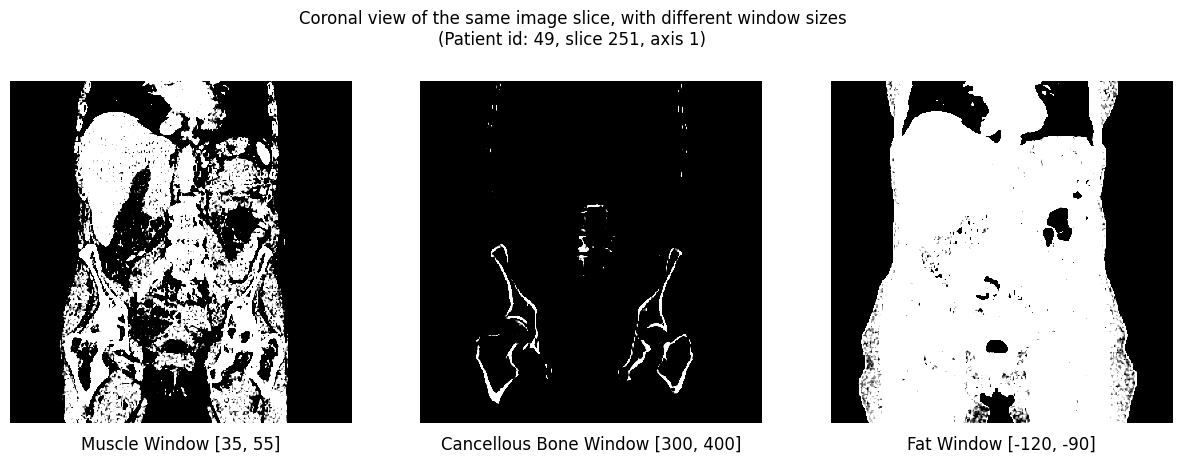
\includegraphics[width=0.3\textwidth, trim=21cm 1cm 0.2cm 2cm, clip]{../figures/HU-window.png}}}
    \caption{Coronal view the same image slice of a CT image, with different window cropping (Patient id: 49, slice 251, axis 1)}
    \label{fig:ct-windows}
\end{figure}

The granularity or image slice thickness is decided by the operator or physician and ranges from 1mm to 10mm. Therefore, the precision along each axis creates a cube, or voxel which represents the value on a grid in three-dimensional space. The voxel values are measured in Hounsfield Units (HU)~\cite{diagnostic-radiology-physics}. 

Contrary to natural images, where pixel values vary from 0 to 255 in 3 channels representing Red, Blue and Green, the Hounsfield scale is a quantitative scale for describing radiodensity where the image intensity reflects tissue type; each voxel intensity refers to specific tissue composition. The positive values are a consequence of more dense tissue with greater X-ray beam absorption, and negative values are less dense tissue with less X-ray beam absorption~\cite{Statpearls}.  

Therefore, becuase the HU scale is relative, different windows may be taken of a CT scan to highlight different tissues. Those voxels that lie within the window, are likely to be tissues of a specific classification. For example, disaplyed in Figure~\ref{fig:ct-windows} we display 3 such windows, muscle, cancellous bone and fat.

\subsection{Data Aquisition}

\subsubsection{Format}

The data acquired through The Royal Marsden Hospital is presented as a set of `Neuroimaging Informatics Technology Initiative' files (NIfTI)~\cite{file-formats}. It serves as a lightweight alternative to other formats such as DICOM and eliminates ambiguity from spatial orientation information~\cite{dicom-to-nifti-conversion}. Libraries exist for handling these files, such as SimpleITK~\cite{SimpleITK-paper} which we use to read and manipulate the data in this project. The library reads, manipulates, and handles the image as a set of points in a grid occupying a physical region in space as defined by the metadata to remove ambiguity from the origin, size, spacing and so on that might vary between patient scans.

\subsubsection{Training Data}

Data was sampled for 100 varying female patients with similar types of cancer. With this data, come 7 relevant segmentation classes which contribute to radiotherapy planning. For the purpose of reproducibility, all delinated lablled data was lablled consistently by the Oncologists to improve chances that an AI model can learn cervical cancer patterns~\cite{AMLART-data}. 

Finally, 10 hold-out data items were provided, which are patients with only the raw CT scan information with no labels.

\subsubsection{Notes}

Some notes contain clinical observations about each of the 100 labelled data pairs~\cite{AMLART-data}. This small sample size of patients is also a good representation of the variability of data in the population. Because of the relatively small sample size, its important to be more acutely aware of the variability in the data. In particular, some observations are summarized.

A common observation is that scans contain poor contrast. For patient 13, the note reads ``no contrast - hard to see LNs'' which is information crutial to determine for segmenting the Clinical Target Volume for Lymph Nodes (CTVn). Additionally, patients 9, 60, and 62 are examples that have ``very large tumors'', sometimes, these even shift into uncommon areas, with ``sigmoid hanging into parametrium''. % GTV not visible?

The notes are helpful to identify and diagnose some reasons for poor performance of the model which is characteristic of the high variability between patients.

\subsection{Delineation classes}

The clinicians at the Royal Marsden Hospital have provided segmentation labels for 5 high-priority classes of interest. These are the Bladder, Anorectum, CTVn, CTVp, and Parametrium.

\subsubsection{Organs At Risk}\label{sec:data-organs-at-risk}

\begin{figure}[H]
  \centering
  \subfigure[Axial]{
    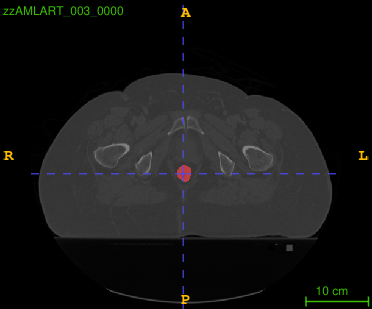
\includegraphics[width=0.3\textwidth]{../figures/PatientStructureExamples/Anorectum_003/Axial.png}
   \label{fig:example-anorectum-axial}
  }
  \subfigure[Coronal]{
    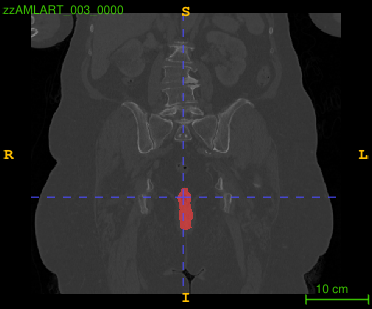
\includegraphics[width=0.3\textwidth]{../figures/PatientStructureExamples/Anorectum_003/Coronal.png}
   \label{fig:example-anorectum-coronal}
  }
  \subfigure[Sagittal]{
    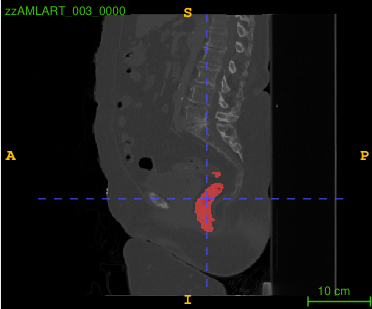
\includegraphics[width=0.3\textwidth]{../figures/PatientStructureExamples/Anorectum_003/Sagittal.png}
   \label{fig:example-anorectum-sagittal}
  }
  \caption{Views of a segmented (in red) Anorectum of an arbitrary patient}
\end{figure}

\begin{figure}[H]
  \centering
  \subfigure[Axial]{
    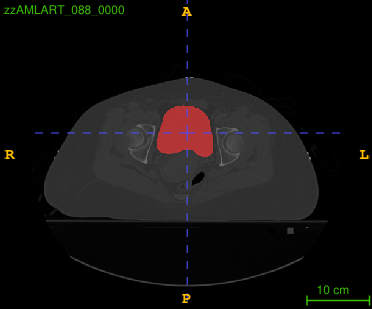
\includegraphics[width=0.3\textwidth]{../figures/PatientStructureExamples/Bladder_088/Axial.png}
   \label{fig:example-bladder-axial}
  }
  \subfigure[Coronal]{
    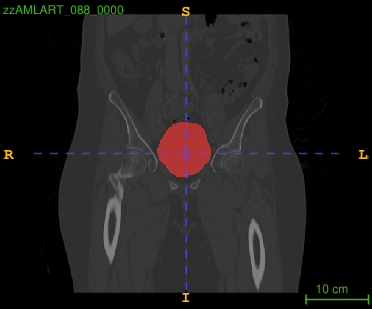
\includegraphics[width=0.3\textwidth]{../figures/PatientStructureExamples/Bladder_088/Coronal.png}
   \label{fig:example-bladder-coronal}
  }
  \subfigure[Sagittal]{
    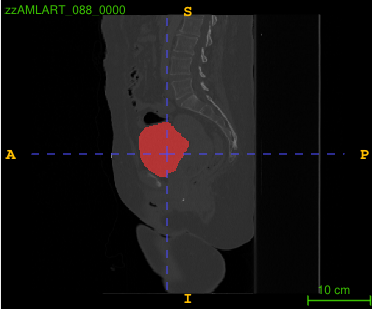
\includegraphics[width=0.3\textwidth]{../figures/PatientStructureExamples/Bladder_088/Sagittal.png}
   \label{fig:example-bladder-sagittal}
  }
  \caption{Views of a segmented (in red) Bladder of an arbitrary patient}
\end{figure}

An organ at risk is an organ which has a substantial probability of being within the PTV despite being healthy. Any areas that are created around the area should actively avoid these organs because by overlapping with them we risk complicating the treatment and compromising the health of functioning organs.

Many anatomies have been provided in the risk categories, however, in particular we have been supplied with contours for the Bladder (Figure~\ref{fig:example-bladder-axial}-\ref{fig:example-bladder-sagittal}) and the Anorectum (Figure~\ref{fig:example-anorectum-axial}-\ref{fig:example-anorectum-sagittal}). In particular, clinicians have identified that the Bladder may overlap with the CTVn (Section~\ref{sec:data-CTVn}) and the Parametrium (Section~\ref{sec:data-Parametrium}).

\subsubsection{CTVp}\label{sec:data-CTVp}

\begin{figure}[H]
  \centering
  \subfigure[Axial]{
    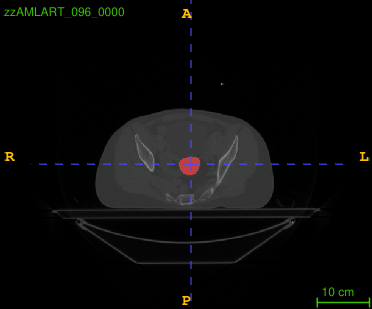
\includegraphics[width=0.3\textwidth]{../figures/PatientStructureExamples/CTVp_096/Axial.png}
   \label{fig:example-CTVp-axial}
  }
  \subfigure[Coronal]{
    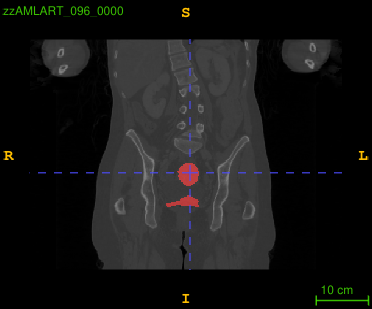
\includegraphics[width=0.3\textwidth]{../figures/PatientStructureExamples/CTVp_096/Coronal.png}
   \label{fig:example-CTVp-coronal}
  }
  \subfigure[Sagittal]{
    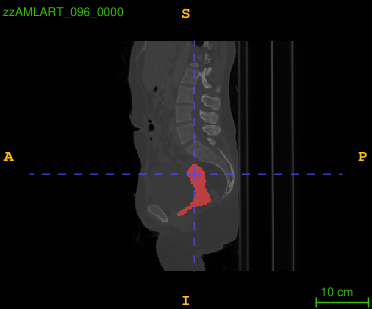
\includegraphics[width=0.3\textwidth]{../figures/PatientStructureExamples/CTVp_096/Sagittal.png}
   \label{fig:example-CTVp-sagittal}
  }
  \caption{Views of a segmented (in red) CTVp of an arbitrary patient}
 \label{fig:example-CTVp}
\end{figure}

The CTVp stands for the Primary Clinical Target Volume, see the example at Figure~\ref{fig:example-CTVp}. This is the CTV where there may be local microscopic spread (uterus, cervix, upper vagina, primary tumour)~\cite{AMLART-data}. This is the area that contains the tumour.

This isn't by any means an organ in a body, but rather an area comprised of other components formed by joining other structures together. The CTVp is an area defined in Equation~\ref{eq:ctvp}.

\subsubsection{CTVn}\label{sec:data-CTVn}

\begin{figure}[H]
  \centering
  \subfigure[Axial]{
    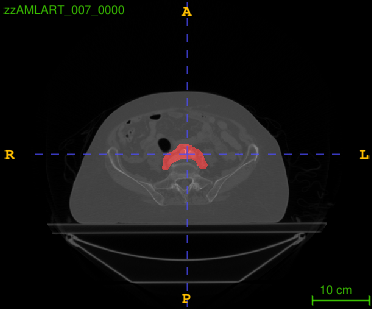
\includegraphics[width=0.3\textwidth]{../figures/PatientStructureExamples/CTVn_007/Axial.png}
   \label{fig:example-CTVn-axial}
  }
  \subfigure[Coronal]{
    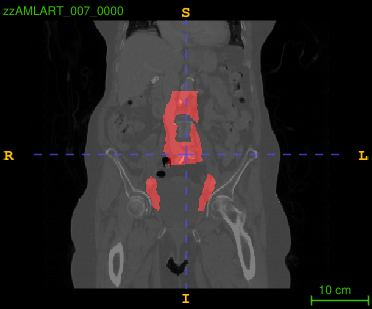
\includegraphics[width=0.3\textwidth]{../figures/PatientStructureExamples/CTVn_007/Coronal.png}
   \label{fig:example-CTVn-coronal}
  }
  \subfigure[Sagittal]{
    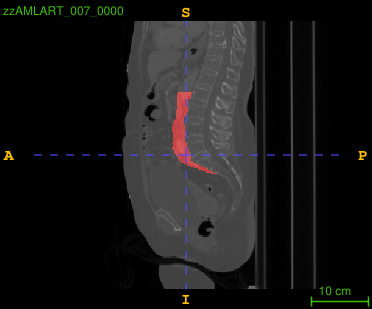
\includegraphics[width=0.3\textwidth]{../figures/PatientStructureExamples/CTVn_007/Sagittal.png}
   \label{fig:example-CTVn-sagittal}
  }
  \caption{Views of a segmented (in red) CTVn of an arbitrary patient}
 \label{fig:example-CTVn}
\end{figure}

The CTVn stands for Nodal Clinical Target Volume, see the example at Figure~\ref{fig:example-CTVn}. This is the CTV where there may be microscopic spread to lymph nodes. It is drawn based on set margins around pelvic blood vessels and includes pelvic lymph nodes, common iliac lymph nodes and para-aortic lymph nodes~\cite{AMLART-data}.

Similarly to CTVp, this is a compound area with three groups of lymph nodes. In clinical practice, the number of these groups included in the CTV varies in each patient, depending on how advanced the disease is. Pathological lymph nodes (GTVn) are also included. The CTVn is an area defined in Equation~\ref{eq:ctvn}.

\subsubsection{Parametrium}\label{sec:data-Parametrium}

\begin{figure}[H]
  \subfigure[Axial]{
    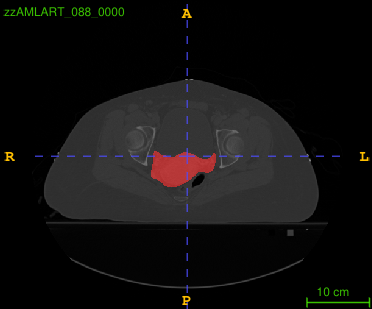
\includegraphics[width=0.3\textwidth]{../figures/PatientStructureExamples/Parametrium_088/Axial.png}
   \label{fig:example-Parametrium-axial}
  }
  \subfigure[Coronal]{
    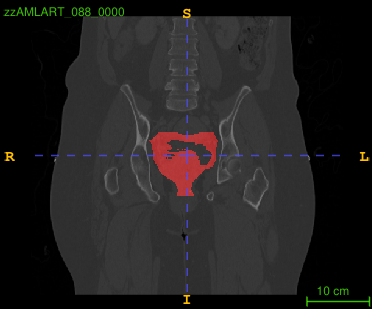
\includegraphics[width=0.3\textwidth]{../figures/PatientStructureExamples/Parametrium_088/Coronal.png}
   \label{fig:example-Parametrium-coronal}
  }
  \subfigure[Sagittal]{
    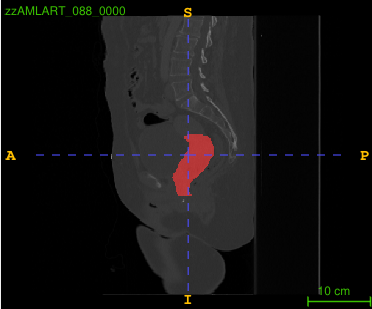
\includegraphics[width=0.3\textwidth]{../figures/PatientStructureExamples/Parametrium_088/Sagittal.png}
   \label{fig:example-Parametrium-saggital}
  }
  \caption{Views of a segmented (in red) Parametrium of an arbitrary patient}
 \label{fig:example-Parametrium}
\end{figure}

The Parametrium (or Paravagina) is the tissue surrounding the cervix/vagina - at risk of local spread, see Figure~\ref{fig:example-Parametrium}. Drawn as a complete structure and editing back to the level of vagina to be included~\cite{AMLART-data}.

\subsection{Rules}\label{sec:data-delineation-rules}

\begin{minipage}{0.5\textwidth}
  \subsubsection{Notation of Structures}
  \begin{enumerate}
    \item Let the Anorectum be denoted as $A$
    \item Let the Bladder be denoted as $B$
    \item Let the Cervix be denoted with $C$
    \item Let the CTVn be denoted with $C_n$
    \item Let the CTVp be denoted with $C_p$
    \item Let the GTVp be denoted with $G_p$
    \item Let the GTVn be denoted with $G_n$
    \item Let the Pelvic Lymph Node be denoted as $L_p$
    \item Let the Common Iliac Lymph Node be denoted as $L_i$
    \item Let the Para-aortic Lymph Node be denoted as $L_{pa}$
  \end{enumerate}
\end{minipage}%
\begin{minipage}{0.5\textwidth}

  \begin{enumerate}
    \setcounter{enumi}{10}
    \item Let the Parametrium be denoted with $P$
    \item Let the Uterus be denoted with $U$
    \item Let the Vagina be denoted with $V$
  \end{enumerate}

  \subsubsection{Relationship between Structures}

  \begin{enumerate}
    \item Let $O$ denote the set $O = \{B, A, C_n, C_p, P \}$ for a particular patient. If we want to talk about a specific patient, we should use the super-script notation to differentiate patients, e.g., $O^i = \{B^i, A^i, C_n^i, C_p^i, P^i\}$.
    \item Let the overlap of two structures be denoted by the set intersect symbol $\cap$.
    \item Let the joint area of two structures be denoted by the set union symbol $\cup$.
  \end{enumerate}

  % \vspace{4em}

\end{minipage}

The top 5 priority structures have been selected to identify and plan an area where radiotherapy should be used. With these structures, there are rules that the clinicians have outlined, they are quoted for clarification (these structures only refer to each independent patient):

\begin{enumerate}
  \item There should be no overlap between the CTVn, CTVp or Anorectum.

        \begin{equation}
          \forall{i,j \in \{C_n, C_p, A\}}\text{ with } i \neq j, i \cap j = \emptyset
        \end{equation}

  \item The Parametrium may overlap with all of the other structures.

        \begin{equation}
          \forall i \in S, \quad P \cap S_i \neq \emptyset \quad \text{(Possibly)}
        \end{equation}

  \item The Bladder may overlap with the CTVn.

        \begin{equation}
          B \cap C_n \neq \emptyset \vee B \cap C_n = \emptyset\label{eq:ctvn}
        \end{equation}

  \item The CTVp is defined as a compound structure containing:

        \begin{equation}
          C_p = \overbrace{C \cup G_p}^{\text{High Risk CTV}} \quad \cup \quad U \cup V\label{eq:ctvp}
        \end{equation}

  \item The CTVn is defined as a compound structure containing:

        \begin{equation}
          C_n = G_n \cup L_i \cup L_p + L_{pa}
        \end{equation}

\end{enumerate}

\section{Technical Context}
\subsection{AI in medical imaging}
\subsection{nnUNet}
\subsection{TotalSegmentator}
\subsection{UniverSeg}
\subsection{SAM}
\section{Evaluation Metrics}

To determine if a contour can be used in a clinical context, would be include calculating the difference between the provided labelled data. However, in a delineation context, we have different ways to evaluate this measure.

Suppose we are writing a linear-regression model to match a line onto a set of points. To quantify the performance of our line we would measure the shortest distance between each point and the predicted line. This relies on the assumption of points in a known domain that a model is attempting to approximate. In this case we are fitting a 1-dimensional model onto 0-dimensional points in the grid space.

% However, it is far harder to decide on a scoring system when in a delineation context. Consider a single slice of a CT-scan with a known contour around the perimeter of a tumour\footnote{Here we assume that the contour will hug the GTV tightly with no concern for microscopic spread around the remainder of the system}. A model like those mentioned in Section~\ref{sect:image-segmentation} would attempt to learn a function to closely replicate the contour. Here our domain, prediction and ground truth are all 2-dimensional objects.

Geometric measures are the most popular, a survey has found~\cite{review-metrics}. These measures compare an auto-contour to a ground-truth contour and return a relative score based on its performance.

\subsection{Classification Based}\label{sect:classification-based}

Assesses if voxels within and outside the auto-contour have been correctly labelled~\cite{review-metrics}. To begin, we define 'positive' to mean that the voxel selected is indeed in need of radiotherapy treatment, and 'negative' to mean that the voxel is classified as healthy.

A standard measure of classification is accuracy. It measures the total amount of correct predictions vs the total predictions it made. However, this measure alone isn't enough to fully capture the bias of a model because it doesn't tell you the full story with class-imbalanced data when there isn't an even number between positive and negative labels.

\begin{equation*}
  \text{Accuracy} = \frac{TP + TN}{TP + TN + FP + FN}
\end{equation*}

Better measures are Precision and Recall scores. The Precision (also known as the Positive Predictive Value~\cite{evaluation-metrics}) measures the proportion of predictions that were successfully correct. The Recall (also known as True Positive Rate~\cite{evaluation-metrics}), on the other hand, ``measures the portion of positive voxels in the ground truth that are also identified as positive by the segmentation being evaluated''.

\begin{equation*}
  \text{Precision} = \frac{TP}{TP+FP}, \quad \text{Recall} = \frac{TP}{TP+FN}
\end{equation*}

\subsection{Spatial Overlap Based}\label{sect:spatial-overlap-based}

Similarly to Classification Based metrics in Section~\ref{sect:classification-based}, an Overlap Based metric measures the extent of overlap between an auto-contour and a reference structure~\cite{review-metrics}.

The scores above can be combined into a more general score $F_\beta$ to give

\begin{equation*}
  \text{F}_\beta = (1+\beta^2)\cdot \frac{\text{Precision} \cdot \text{Recall}}{\beta^2 \cdot \text{Precision}+\text{Recall}}
\end{equation*}

A specific case of this equation with $\beta=1$ is mathematically equivalent to the DICE Similarity Coefficient which was found to be the most popular evaluation metric amongst 2021 studies~\cite{review-metrics,evaluation-metrics, Sherer2021-le}.

% \begin{align*}
%   F_1 = \text{DICE} & = \frac{2 \cdot \text{Precision} \cdot \text{Recall}} {\text{Precision} + \text{Recall}} & \\ 
%   % & = \frac{2 \cdot \frac{TP}{TP + FP} \cdot \frac{TP}{TP + FN}}{\frac{TP}{TP + FP} + \frac{TP}{TP + FN}} \\
%   % & = \frac{2 \cdot TP \cdot TP}{TP(TP+FN)+TP(TP+FP)} \\ 
%   & = \frac{2 \cdot TP}{2TP + FP + FN} \quad = \quad \frac{2|S_g^1\cap S_p^1|}{|S_g^1|+|S_p^1|} , \text{where} \begin{cases}
%     S_g^1 & \text{ground truth} \\
%     S_p^1 & \text{segmentation}
%   \end{cases}
% \end{align*}

\begin{equation*}
  F_1 = \text{DICE} = \frac{2 \cdot \text{Precision} \cdot \text{Recall}} {\text{Precision} + \text{Recall}} = \frac{2 \cdot TP}{2TP + FP + FN} \quad = \quad \frac{2|S_g\cap S_p|}{|S_g|+|S_p|}
\end{equation*}

Where $S_g$ is the ground truth segmentation and $S_p$ is the predicted segmentation. From this relationship, the DICE score has found popularity in image segmentation for similar reasons that the $F_1$ score has found its popularity classical machine learning; it is able to provide a fair result for imbalanced datasets. This mentality is applicable in our scenario because a tumour will make up very little of the total volume of the domain space. This can be extended to a Volumetric DSC by considering the above in all 3-dimensions~\cite{APL}.

Another popular related evaluation method is the Jaccard Index, which measures the intersection over the union of two sets:

\begin{equation*}
  \text{JAC} = \frac{TP}{TP+FP+FN} = \frac{|S_g\cap S_p|}{|S_g \cup S_p|} \iff \frac{DICE}{2 - DICE}
\end{equation*}

Since the numerator for the Jaccard Index is smaller (since we avoid the issue of counting the intersecting sections twice) the JAC is always larger than the DICE score.

\subsection{Surface Based}\label{sect:surface-based}

Also commonly known as Boundary-Distance-Based Methods~\cite{boundary-overlap-metrics} compares the distance between two structure
surfaces. These can be either maximum distance, average distance or distance at a set percentile of ordered distances~\cite{evaluation-metrics}.

A common example is the Haussdorf Distance. Here, a directed distance metric is defined as the maximum distance from a point in the first set to a nearest point in the other between two individual voxels~\cite{boundary-overlap-metrics}. Therefore, the better the HD metric, the smaller the value it returns. Here, the distance is taken by some norm, typically Euclidian distnace.

\begin{equation*}
  \text{HD}(A,B) = \max(h(A,B), h(B,A)), \quad \text{ and directed h}(A,B)=\max_{a\in A}\min_{b \in B} ||a-b||
\end{equation*}

The HD is generally sensitive to outliers. Because noise and outliers are common in medical segmentations, it is not recommended to use the HD directly~\cite{boundary-overlap-metrics}. Therefore, we can calculate the average directed Haussdorf Distance.


\subsection{Volume Based}

Volume-based metrics consider only the volume of the segmentation~\cite{evaluation-of-metrics-in-prostate,review-metrics, boundary-overlap-metrics}. However, due to its poor spatial descriptions it is more commonly used jointly with other metrics.

\begin{equation*}
  \text{Relative Volume Difference (RVD)} = \bigg| \frac{|S_g|-|S_p|}{|S_g|}\bigg|
\end{equation*}

\subsection{Evaluation}\label{sect:evaluation-of-evaluation-methods}

All these methods can be advantageous in some places rather than other. We can begin to list off some challenging scenarios to decide which segmentation is the best.

\begin{figure}[H]
  \centering
  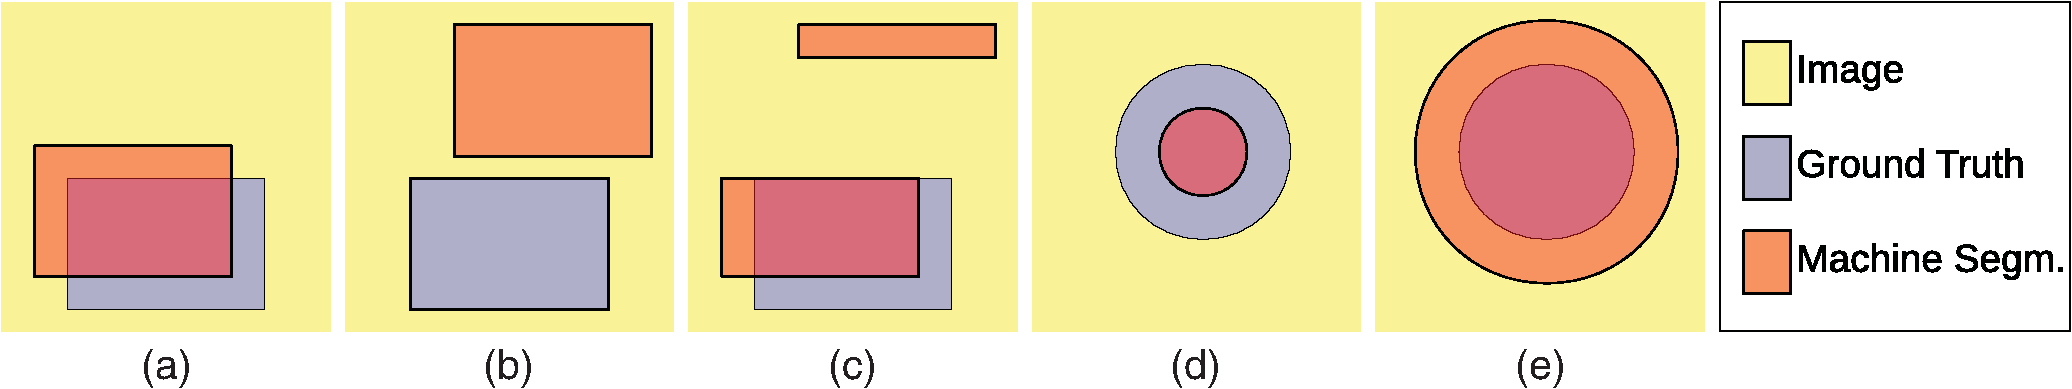
\includegraphics[width=\linewidth]{../figures/segmentation-cases-1.png}
  \caption{Figure from~\cite{boundary-overlap-metrics} illustrating cases of segmentation to aid with explanation of set-backs of certain evaluation metrics}
 \label{fig:segmentation-cases-1}
\end{figure}

\begin{itemize}
  \item Classification Based (Section~\ref{sect:classification-based}) and Spatial Overlap Based (Section~\ref{sect:spatial-overlap-based}) are similar; they are concerned with the number of correctly classified or misclassified voxels without taking into account their spatial distribution. Here, Figure~\ref{fig:segmentation-cases-1}(a) and Figure~\ref{fig:segmentation-cases-1}(c) would achieve similar results despite Figure~\ref{fig:segmentation-cases-1}(a) being locally bound to a better area.
  \item With Haussdorf Distance (Section~\ref{sect:surface-based}) output segmentations generated by Figure~\ref{fig:segmentation-cases-1}(d) and Figure~\ref{fig:segmentation-cases-1}(e) will result in the same score, which is not favorable in a radiotherapy planning environment where an organ-at-risk is involved.
  \item Figure~\ref{fig:segmentation-cases-1}(b) would score flawlessly when using volumetric score estimation, however, it doesn't take into acount spatial placement, which makes this measurement rather poor when used individually.
\end{itemize}

\subsection{Estimated Editing Based}\label{sect:surface-dice}

\begin{warning}
  This is a quotation from this paper,~\cite{Sherer2021-le}, however, it is referencing a paper of its own. Shall I reference the original paper or are 'linked' references OK?
\end{warning}

It is difficult to select a measurement which can reflect a clinicians acceptability score. A study found that there was a lack of correlation between a geometric index and expert evaluation, with the JAC score having a 13\% False Positive Rate. The conclusion of the study summarised that scores such as JSC and volumetric DSC, ``provide limited clinical context and correlation with clinical or dosimetric quality''~\cite{Sherer2021-le}.

% Because of the clinical context of evaluating the segmentation by a machine, it may sometimes be helpful to define a performance metric as the ``fraction of the surface that needs to be redrawn''~\cite{Nikolov2021-xe} since models at this point require manual review to avoid automation bias (Section~\ref{sect:using-the-tool}). For larger structures, this method is useful it doesn't assign a lot of weight on the large trivial internal volume which accounts for a much larger proportion of the score.

\subsubsection{Surface DSC}\label{sect:surface-DSC}

The study at~\cite{Sherer2021-le} helped drive an initiative to combine aspects of Surface Based evaluation (Section~\ref{sect:surface-based}) and Spatial Overlap Based evaluation (Section~\ref{sect:spatial-overlap-based}) into a Surface DICE. This assesses the specified tolerance instead of the overlap of the two volumes.

\begin{figure}[H]
  \centering
  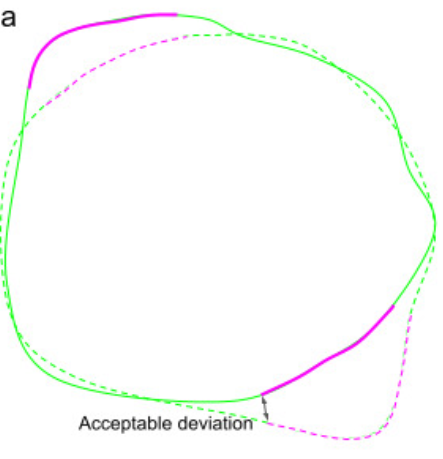
\includegraphics[width=0.3\linewidth]{../figures/Surface-dice.png}
  \caption{Taken from~\cite{Nikolov2021-xe}. Illustrates the computation of the surface DICE, where the continuous line is the predicted surface and the dashed line is the ground truth. The black arrows show the maximum deviation tolerated without penalty; therefore, in pink is the unacceptable deviations and green otherwise.}
\end{figure}

We can formulate the Surface DSC score in a mathematical definition~\cite{Sherer2021-le}.

\begin{equation*}
  \text{Surface DSC} = \frac{|S_p \cap B_{g,\tau}| + |S_g \cap B_{p,\tau}|}{|S_p| + |S_g|}
\end{equation*}

Which provides a measure of the agreement between just the surfaces of two structures above a clinically determined tolerance parameter, $\tau$. Here, $B_{p,\tau}$ represents the  boundary region of the predicted surface within a maximum margin of deviation $\tau$ and similarly for $B_{g,\tau}$ for the ground truth.

\subsubsection{Added Path Length}

In a similar spirit, the APL was proposed as a score to predict ``the path length of a contour that has to be added''~\cite{APL}. This is achieved similarly by considering the number of added voxels required between the prediction and the gold standard with no regard to tolerance as a pose to Surface DSC (Section~\ref{sect:surface-DSC})

\begin{warning}
  For future reference, \textit{\href{https://stackoverflow.com/questions/73286639/how-to-calculate-added-path-length-apl-image-segmentation-metric}{stack overflow discussion}}

  Implementation of surface DSC and APL: \textit{\href{https://github.com/pyplati/platipy/blob/master/platipy/imaging/label/comparison.py}{source code}}
\end{warning}

\subsection{Summary}

This is why we settle at the Surface DSC (Section~\ref{sect:surface-dice}) which prioritizes deviation along boundary to a certain degree while measuring the fraction of the surface that needs to be redrawn, thus favouring a more conservative prediction of Figure~\ref{fig:segmentation-cases-1}(d) instead of (e).

For the purpose of this project, we shall select a evaluation measurement which is more bias towards conservative boundary estimates to not touch the organs at risk. This choice was in-part influenced by the clinician's review pipeline; it would easier to correct Figure~\ref{fig:segmentation-cases-1}(d) instead of Figure~\ref{fig:segmentation-cases-1}(e) because correcting the latter would likely take a considerable amount of time as it would require redrawing almost all of the boundary, whereas the former could be corrected much faster~\cite{Nikolov2021-xe}.



%%%%%%%%%%%%%%%%%%%%%%%%%%%%%%%%%%%%
\chapter{Methodology}

\section{Base-line nnUNet...}

%%%%%%%%%%%%%%%%%%%%%%%%%%%%%%%%%%%%
\chapter{Results}

...

%%%%%%%%%%%%%%%%%%%%%%%%%%%%%%%%%%%%
\chapter{Discussion}

Here, discuss results from all 4 of the methods tested.

%%%%%%%%%%%%%%%%%%%%%%%%%%%%%%%%%%%%
\chapter{Conclusion}

Transfer works!

%%%%%%%%%%%%%%%%%%%%%%%%%%%%%%%%%%%%
\chapter{Ethics}

The lack of effort to protect the identities and confidentiality of patients during research projects may result in ``stigma, embarrassment, and discrimination''~\cite{health-privacy} if the data is misused.
This project involves very intimate and personal information of many female patients whose privacy must be established concretely before research is to take place.%. Researchers may collaborate with third-parties such as Imperial College London by providing anonymized data which may not be reverse engineered back to the patient.

\section{Patient disclosures}

Reserachers may collaborate with third-parties such as Imperial College London by providing anonymized data which may not be reverse engineered back to the patient. The collaborating hospital, The Royal Marsden Hospital, doesn't require ``explicit consent'' for sharing collected clinical data with outside entities as long as the patient is made aware of the ways their ``de-identified/anonymized'' data may be used.~\cite{royal-marsden-privacy-note}. Formalities are also arranged with Imperial Collage's Medical Imaging team such as acting as ``ethical data stewards''~\cite{Larson2020-ib}. Without such disclosure and anonymisation of data, patients may be reluctant to provide candid and complete disclosures of their sensitive information, even to physicians, which may prevent a full diagnosis if their data isn't maintained in an anonymous fashion.

The MIRA team acts as responsible data stewards by storing anonymized data within a folder on the college network. All provided data was anonymized by the Royal Marsden Hospital and sent to team MIRA in the \texttt{NIfTI} file format which discloses no personal identifiable information, as defined by GOV website~\cite{gov-gdpr}. This folder contains security measures which limit the availability of data only to those with specific access rights. Furthermore, operating on the preamble of de-identified data further reduces individual patient risk in the event that data is ever brought outside the confines of this folder.

\section{Using the tool}\label{sect:using-the-tool}

The applications of this tool bode well in the healthcare ecosystem as the community slowly accepts the involvement of AI-powered medical tools. Radiology has been one application that has been most welcoming of the new advances in technology as there is potential for substantial aid by reducing manual labor, increasing precision and freeing up the primary care physician's time~\cite{Amisha2019-ki}.

Yet, it is too early to take result the medical tool as gospel. For current cervical radiotherapy delineation tools, only 90\% of the output is considered as acceptable for clinical use~\cite{LIU2020172}. The remainder therefore has the potential to cause more harm than good if not checked properly. For example, overlap of a PTV onto an organ-at-risk may invoke a cascade of negative effects for the patient. A physician may base their final judgement subject to a multivariate analysis, which is contrary to the single image modality that this tool is based on. Therefore, the tool should be used as a second opinion rather than a primary source of information.

Clinicians can fall into the trap of automation-bias as AI becomes more common place in clinical environments~\cite{STRAW2020101965}. However, many models of this age codify the existing bias in common cases, which often will fail those patients who do not fit the expectations of the majority. Therefore, a degree of supervision required from physicians has to be established if this tool is to be used in practice. Oncologists will be required to reverse-engineer results of the `black-box' to verify why a decision has been made. Secondly, the responsible party for incorrect decisions made by DL tools should also be determined~\cite{Chen2021-dg}.

%%%%%%%%%%%%%%%%%%%%%%%%%%%%%%%%%%%%

%% bibliography
\bibliography{../.latex-templates/references}

\end{document}